\documentclass[10pt,a4paper]{scrartcl}
\usepackage[utf8x]{inputenc}
\usepackage{amsmath}
\usepackage{amsfonts}
\usepackage{amssymb}
\usepackage{listings}
\usepackage{pdfpages}
\usepackage{url}
\usepackage[colorlinks=true,linkcolor=black]{hyperref}
\usepackage[T1]{fontenc}
\usepackage[ngerman]{babel}
\usepackage[left=2cm, top=2cm,right=2cm,bottom=2cm]{geometry}

% \ifpdf
%   \usepackage[pdftex]{graphicx}
% \else
%   \usepackage[dvips]{graphicx}\fi

\begin{document}

\newcommand{\Version}{1.2}


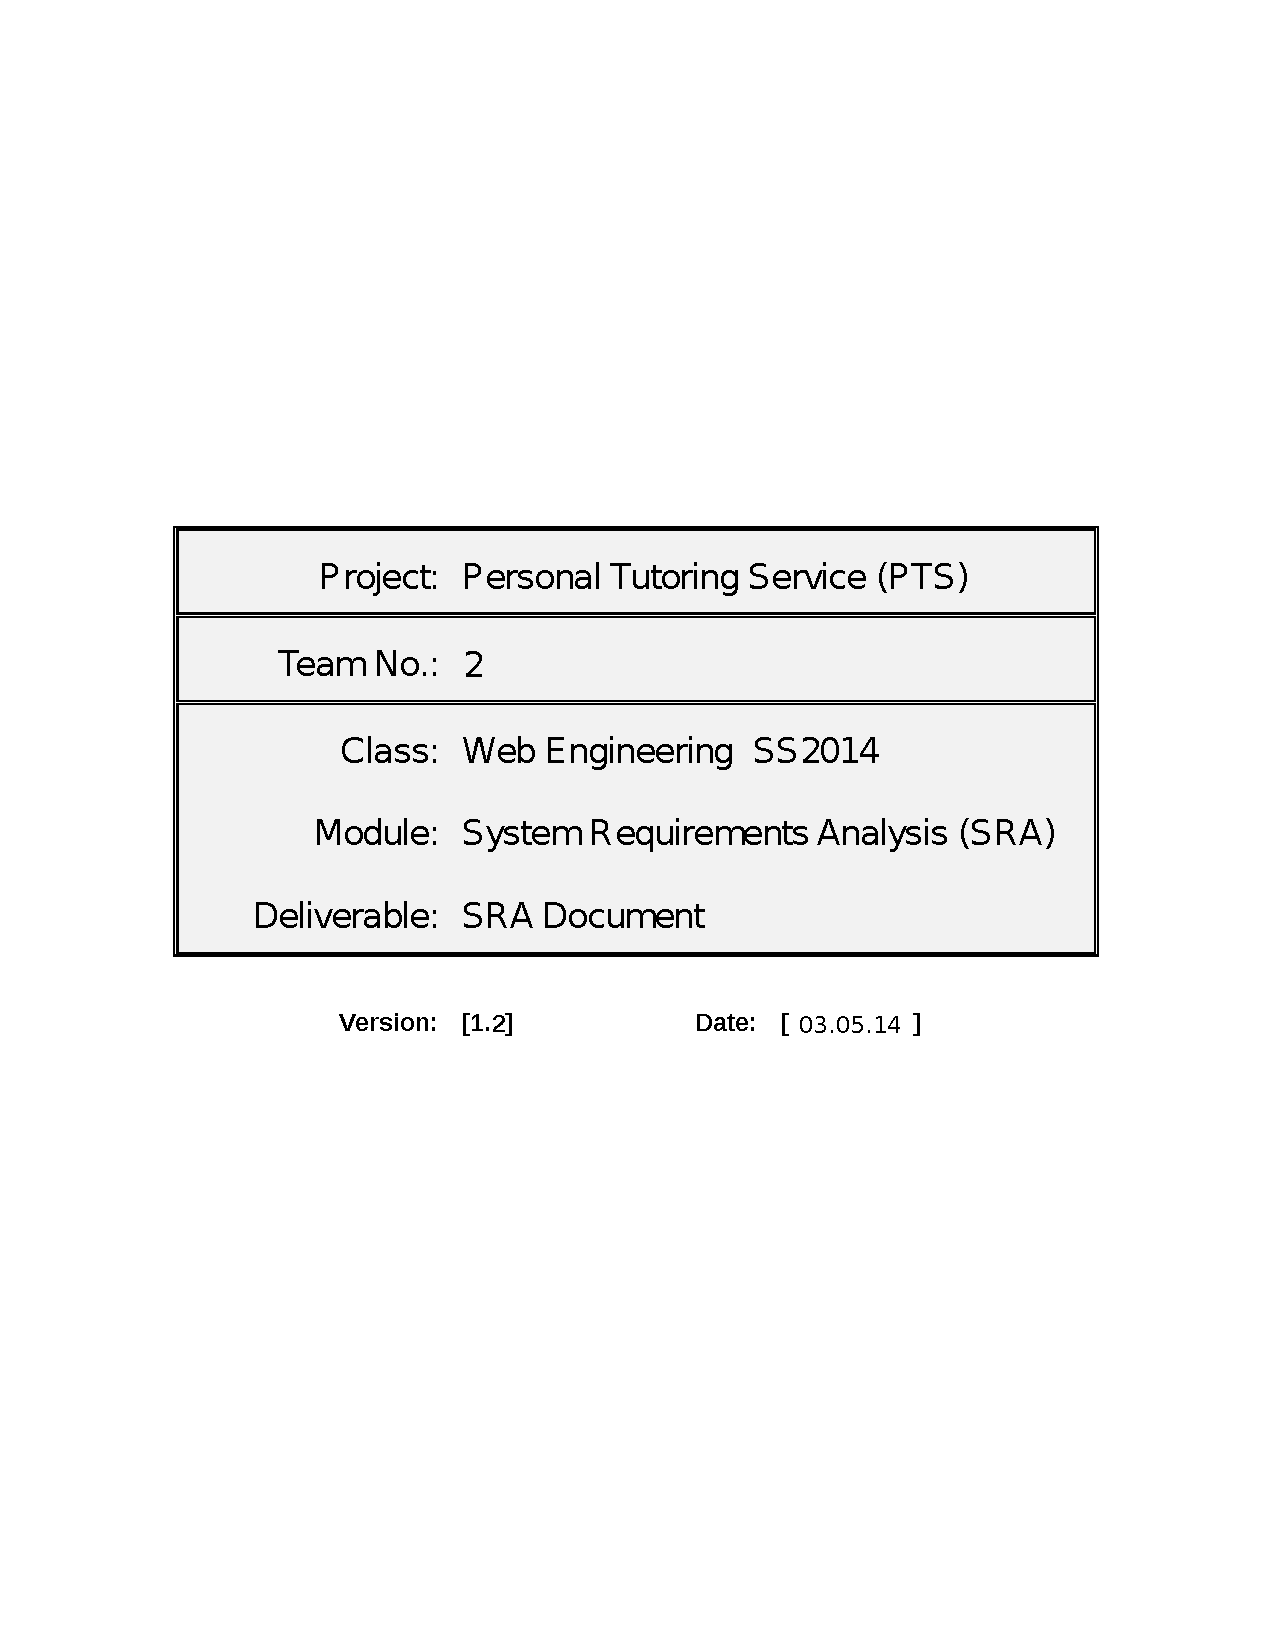
\includepdf{SRA_Titelblatt.pdf}



\newpage
\begin{itemize}
\item[] \textbf{\large Beitragende:}\\
Sven Liebl\\
Matthias Goetz\\
Christian Dauerer\\
Maxmilian Schröter\\
Stefan Holz - aus Team ausgetreten\\
Viet Nguyen - aus Team ausgetreten \\
Daniel Tatzel\\
Nils Weiss\\
Florian Laufenböck\\
Alexander Strobl\\
Matthias Birnthaler\\
Tobias Schwindl
\end{itemize}

\bigskip

\begin{table}[!h]
 	\centering
	\begin{tabular}{|c|c|c|c||c|}
	\hline
	\textbf{VersionsNr} &  \textbf{Datum} & \textbf{Auslöser} & \textbf{Veränderungsgrad} & \textbf{Beschreibung} \\
	\hline
	1.0 & 03.04.2014 & Strobl & Erster Entwurf & Initial Release \\
	\hline
	1.1 & 11.04.2014 & Strobl & Verbesserungen & neue Features \\
	\hline
	1.2 & 03.05.2014 & Tatzel & Anpassung & Features Entf. \\
	\hline
	1.3 & 07.05.2014 & Strobl & Anpassung & Kontextdiagramme \\
	\hline
	1.4 & xx.06.2014 & Alle & Anpassung & Final Release \\
	\hline
	\end{tabular}

\caption{Überarbeitungshistorie}
\end{table}

\newpage
\tableofcontents
%\listoftables


\newpage
\section{F: Funktionale Anforderungen}


\subsection{F1: Öffentlicher Bereich}
\subsubsection*{F11: Startseite}

Informiert den Besucher über Funktion und Zweck der Webseite. Ebenfalls wird eine Karte mit der Route zum Hauptsitz der Tutoren AG in Deutschland implementiert. Ein Teaser über das Motto und der Angebote der Website soll den Besucher ansprechen und so sein Interesse fördern. Durch die Anzeige von Top Gästebucheinträgen wird dem Gast das Gefühl der Vertrauenswürdigkeit und der Kompetenz übermittelt.

\subsubsection*{F12: Gästebuch}

Im Gästebuch können eingeloggte Besucher ihre Kommentare über den Service hinterlassen. Bevor es im Gästebuch erscheint, muss es vom Administrator freigegeben werden, um Falschaussagen zu vermeiden.

% \subsubsection*{F13: Anzeige von verfügbaren Tutoren in der Nähe}
% Anhand einer Wohnortsuche ist im Voraus überprüfbar, ob Tutoren in der Nähe zu finden sind.

% \subsubsection*{F14: Erweiterte Suchkriterien}
%
% Beinhalten die Suche der gewünschten Schulart, Fach, Klasse, Preis und die maximale Fahrzeit zwischen Tutoren und Schülern.

\subsubsection*{F13: Registrierungs- und Anmeldefenster}

Um den kompletten Serviceumfang ausnutzen zu können, ist eine Anmeldung bzw. Registrierung nötig.

\subsubsection*{F14: About us (Impressum)}

Das Impressum enthält folgende Informationen: Firma, Straße, Postleitzahl, Ort, Telefonnummer, E-Mailadresse, Internetadresse, Vertretungsberechtigter, \\ Geschäftsführer, Inhaltlich Verantwortlicher und Haftungshinweis.

% \subsubsection*{F17: Preismodell/Zahlungsinfos}
%
% Informiert vorab über die Zahlungshinweise und Preise, um Irrtümer zu vermeiden.

\subsubsection*{F15: Auswahl der Sprache}

Dem Besucher ist es möglich, zwischen Deutsch und Englischer Sprache auszuwählen. Diese Option unterstützt die Benutzerfreundlichkeit für Besucher außerhalb des deutschsprachigen Raumes.

\subsubsection*{F16: Support und Kontaktdaten}

Persönliche Hilfen oder Anfragen, sind an den Support zu stellen. Erreichbar ist der Support \"uber die Angaben auf der Support Seite.


\subsection{F2: Administrator}

\subsubsection*{F21: Anmelden}

Der Administrator meldet sich mit einem Nutzernamen und einem Passwort an, um den privaten Adminbereich betreten zu können.

\subsubsection*{F22: Persönliche Einstellungen}

Wie jeder Nutzer verfügt der Administrator über ein persönliches Profil welches Nutzername, Name, Vorname, E-Mail , Geburtsdatum, Postleitzahl, Wohnort, Straße, 
Hausnummer und Telefon enthält. Es ist nicht möglich alle Profilinformationen zu Bearbeiten. Nutzername, Name, Vorname und Geburtsdatum sind von einer Bearbeitung ausgeschlossen.
Alle anderen Informationen sind mit entsprechende Masken und Formularen editierbar. Es besteht die Möglichkeit das Profil zu löschen.

\subsubsection*{F23: Adminverwaltung}

Der Administrator kann Kundendaten einsehen. Er kann Kundenkonten löschen. Des Weiteren muss er neue User-Accounts freischalten.
Neue Gästebucheinträge werden dem Administrator angezeigt/gemeldet und erst nach seiner Freischaltung veröffentlicht.
Der Admin hat die Möglichkeit Nachrichten zu löschen.

\subsubsection*{F24: Nachrichten}
Wenn der Administrator die Nachrichtenseite aufruft kann er mittels von Formularen neue Nachrichten verfassen.

% \subsubsection*{F24: Zugriff auf Nachrichtensystem}
%
% Der Administrator kann Nachrichten an die Nutzer versenden und welche von diesen erhalten. Ungelesene Nachrichten werden angezeigt.

%\subsubsection*{F24: Freischaltung von Gästebucheinträge}

%Neue Gästebucheinträge werden dem Administrator angezeigt/gemeldet und erst nach seiner Freischaltung veröffentlicht.

\subsubsection*{F25: Abmelden}

Der Administrator kann sich abmelden und es stehen ihm nur noch die Funktionalitäten des öffentlichen Bereiches zur Verfügung.

\subsubsection*{F26: Besucherzähler}

Zählt die Anzahl der der Leute, die die Seite besucht haben. Dadurch kann die Popularität der Website ermittelt werden.
Der Zähler wird bei jedem Startseitenaufruf erhöht.

\subsubsection*{F27: Privater Ordner}
Der Adimistrator hat Zugriff auf einen privaten Ordner, den bei dem er sich mit einem extra Benutzernamen und Passwort anmeldet. Hier kann er Dokumente 
Dort kann er Dokumente Up- und Downloaden und diese ensehen.

\bigskip

$^1$ Kundenkonten: Tutorenkonten und Schülerkonten\\
$^2$ Kundeninformationen: Persönliche Informationen der Kundenkonten




\subsection{F3: Schüler}
Jeder Besucher hat die Möglichkeit ein Profil anzulegen und sich mit den erhaltenen Zugangsdaten einzuloggen.
Dadurch erhält er Zugriff auf seinen Privaten Bereich, in dem er seine bei der Registrierung hinterlegten persönlichen Daten ändern kann.
Die persönlichen Daten setzen sich aus Vorname, Nachname, Alter, Anschrift, Passwort und Kontaktdaten zusammen.
Es besteht die Option seinen Account zu löschen.

% \subsubsection*{F31: Detaillierte Suche}
%
% Im Gegensatz zum nicht registrierten Besucher besitzt der Anwender die Möglichkeit einer detaillierten Suche nach folgenden Kriterien: Lehrer, Ort, Fach.

\subsubsection*{F31: Schülerprofil}

Der registrierte Anwender ist berechtigt das Profil des Schülers einzusehen, das für den Anwender folgende Informationen bereit hält:

\begin{itemize}
	\item Geschlecht
	\item Stundenlöhne
% 	\item Verfügbarkeiten
	\item Fächer / Jahrgangsstufen
	\item Verfügbare Orte / Regionen
% 	\item Profilbild
	\item Kontaktdaten
% 	\item Lehrerbewertung
\end{itemize}

% Er ist in der Lage das Schwarze Brett des Tutors einzusehen.


\subsection{F4: Lehrer / Tutor}
\subsubsection*{F41 Profil einstellen}
Der Tutor kann ein Profil erstellen, um sich kurz vorzustellen und Werbung in eigener Sache machen zu können.

Das Profil soll beinhalten / anbieten:
\begin{itemize}
	\item Stundenlöhne verlangen
% 	\item Verfügbarkeiten angeben
	\item Fächer / Jahrgangsstufen einstellen
	\item Verfügbare Orte / Regionen anbieten
% 	\item Zahlungsdaten zur Verfügung stellen
% 	\item Sieht in einer Übersicht seine Schüler und einen Kalender mit den nächsten Terminen
% 	\item Rechnungen / Zahlungserinnerungen verschicken
% 	\item Profilbild
	\item Kontaktdaten
% 	\item Lehrerbewertung / Gästebuch
\end{itemize}

% \subsubsection*{F42 Schwarzes Brett}
%
% Der Tutor kann allgemeine Informationen hinzufügen z.B. bei Krankheit.

% \subsubsection*{F43: Zugriff auf Nachrichtensystem}
%
% Tutoren und Tutoren können Nachrichten an die Nutzer versenden und welche von diesen erhalten. Ungelesene Nachrichten werden angezeigt.

% \subsubsection*{}
% \item[] \textbf{F43 Lehrmaterialien online stellen und verteilen}\\
% Er kann Dateien nach Bedarf für die Schüler per eMail verteilen.
%
% \subsubsection*{}
% \item[] \textbf{F44 Beurteilungen schreiben}\\
% Der Schüler kann Feedback für seine abgegeben Aufgaben / Leistungen erhalten

\subsection{F5: Registrierte Benutzer}

\subsubsection*{F51: Spenden per Kreditkarten}
Jeder registrierte Benutzer kann mit Kreditkarte Spenden. Diese Informationen werden für den nächsten Zahlungsvorgang gespeichert.

\section{S: Systemanforderungen}
Hinweis: Die systembezogenen Anforderungen machen deutlich, welche Voraussetzungen hard- und softwareseitig für den Systemeinsatz gegeben sein müssen.

\subsection{S1: Anforderungen an die Hardware}
\subsubsection*{S11: Datenbankserver}

2 Prozessoren mit einer Taktfrequenz $>$ 1 GHz\\
Arbeitsspeicher mit einer Speicherkapazität $>$ 1GB\\
Festplatten (SCSI): $>$ 500 GByte, RAID 5\\
Backupsystem\\
Antivirensoftware

\subsubsection*{S12: Web- und Applicationserver}

2 Prozessoren mit einer Taktfrequenz $>$ 850 MHz\\
Arbeitsspeicher mit einer Speicherkapazität $>$ 1GB\\
Festplatten(SCSI): $>$ 100 GB, RAID 0\\
Backupsystem\\
Antivirensoftware\\
Firewall

\subsection{S2: Anforderungen an die Systemsoftware}
Da keine Kosten für die Nutzung von Systemsoftware anfallen dürfen und das System Mindestanforderungen an die Datensicherheit und den Datenschutz genügen muss, sind folgende freie Softwarekomponenten zu verwenden:
\begin{itemize}
\item MySQL als relationale Datenbank für die zentrale Datenhaltung
\item Linux als Betriebssystem
\item Apache als Web- bzw. Applicationserver
\item Mailserver zum Verteilen von Lehrmaterialien
\end{itemize}

\subsection{S3: Programmiersprache}
Als Programmiersprachen sind Java-Script, PHP und SQL einzusetzen.


\subsection{S4: Allgemeine Anforderungen an die Webseite}
\begin{enumerate}
\item[] \textbf{Allgemeine Funktionalitäten}
\item Die Webseite ist W3C-Konform zu gestalten
\item Google Analytics wird eingebunden
\item Ein Font für die komplette Webseite
\item Zugriff auf die Webseite ohne "www" vorne
\item Logo
\item Google Webmaster Tools
\item Geolocation soll festgelegt sein
\item URL Rewriting für Suchmaschine
\item Elemente sollen abgerundete Ecken haben
\item Es soll ein Box- und Text-Shadow implementiert werden
\item Private Ordner sind über gesonderte Zugangsdaten erreichbar (Unabhängig vom Benutzer und Login)

\item[] \textbf{Startseite}
\item Auf der Startseite soll ein Video über einen Button gestartet werden
\item Auf der Startseite soll ein Top-Down-Menü zur Verfügung gestellt werden
\item Die Startseite soll eine 3-spalige Ansicht haben
\item Slideshow

\item[] \textbf{Funktionen für alle Benutzer}
\item Eigene 404-Fehlerseite, falls die angeforderte Webseite nicht gefunden wurde
\item Eine Suchmaschine soll Suchfunktionen zur Verfügung stellen, der Umfang der Suchergebnisse hängt von dem Status des Benutzers ab (nicht eingeloggt, Admin, Tutor, Schüler)
\item Suchergebnisse können nach verschiedenen Kriterien sortiert werden
\item Logins sind sessionbasiert
\end{enumerate}



%\subsection{S4: Tools}
%\begin{itemize}
%HTML-Entwicklungsumgebung
%Java- bzw. PHP-Entwicklungsumgebung
%Für die Entwicklung und den Test der Anwendung muss eine %spezielle Testumgebung zur Verfügung gestellt werden.
%\end{verbatim}




\section{Q: Qualitative Anforderungen}
Hinweis: Qualitative Anforderungen spezifizieren nicht-funktionale Anforderungen wie z.B. Ausfallsicherheit, Zuverlässigkeitsanforderungen, Portabilitätsanforderungen sowie gewünschte Antwort- und Verarbeitungszeiten.

\subsection{Q1: Nachweis der Funktionalität}
Die Realisierung der funktionalen Anforderungen ist durch geeignete Tests nachzuweisen.

\subsection{Q2: Gewährleistung von Datenschutz und Datensicherheit}
Aufgabe der Datensicherheit ist es, Unternehmens- und personenbezogene Daten insbesondere vor Verlust oder Missbrauch zu schützen. Eine Datenbank oder Daten sollen geschützt, rekonstruierbar, überprüfbar und einbruchssicher untergebracht sein. Ihre Benutzer sollen identifizierbar und zu bestimmtem Aktionen berechtigt sein. Bei der Verarbeitung personenbezogener Daten sollen die Aktionen protokolliert und überwacht werden. Aufgabe des Datenschutzes ist es, den Einzelnen davor zu schützen, dass er durch den Umgang mit seinen personenbezogenen Daten in seinem Recht beeinträchtigt wird, selbst über die Preisgabe und Verwendung seiner Daten zu bestimmen ("informationelles Selbstbestimmungsrecht"). Dies gilt sowohl für Kunden- als auch für Mitarbeiterdaten. Die Datenschutzmaßnahmen müssen die Einhaltung der gesetzlichen Vorgaben gemäß GG[1], BDSG[2] und BayDSG[3] sicherstellen. Personenbezogene Daten dürfen nur mit Zustimmung der betroffenen Person erhoben werden. Die Speicherung der Daten ist nur solange gestattete, wie die Einwilligung des Betroffenen vorliegt. Es ist nach dem Prinzip der Datenvermeidung zu verfahren. Die Maßnahmen zur Gewährleistung von Datenschutz und Datensicherheit:
\begin{itemize}
	\item[] \textbf{Q21}: die Erarbeitung und Umsetzung eines Berechtigungskonzepts
	\item[] \textbf{Q22}: die Erarbeitung und Umsetzung eines Benutzerkonzeptes für die Datenbank
	\item[] \textbf{Q23}: die Erarbeitung und Umsetzung eines Sicherheitskonzeptes
\end{itemize}
\bigskip
\begin{tabular}{cl}
Referenz & Titel\\
$[1]$ & Grundgesetz (GG)\\
$[2]$ & Bundesdatenschutzgesetz (BDSG)\\
$[3]$ & Landesdatenschutzgesetz Bayern (BayDSG)
\end{tabular}


\subsection{Q3: Benutzerfreundliche Oberfläche}
Es ist eine benutzerfreundliche Oberfläche zu schaffen. Der Einsatz von Orien-tierungs-, Navigations-, Inhalts-, Layout- und Interaktionselementen hat so zu erfolgen, dass der Benutzer sie intuitiv erfassen und effektiv benutzen kann. Der Nachweis ist durch die Einbeziehung einer unabhängigen Benutzergruppe bei unsystematischen Tests und anschließender Interview zu erbringen. Den Benutzern wird ferner eine Online-Hilfe zur Verfügung gestellt, die einer Benutzerdokumentation in Art und Umfang entspricht.


\subsection{Q4: Zuverlässigkeit}
Für eine gute Akzeptanz beim Benutzer einer Web-Applikation ist ein hoch verfügbares (98$\%$) und stabiles System erforderlich. Der Nachweis ist durch entsprechende Messungen zu führen. Es ist ein skalierbares System (Clusterbildung, Loadbalancing) zur Verfügung zu stellen.


\subsection{Q5: Effizienz}
Das Antwortzeitverhalten ist so zu beeinflussen, dass nicht mehr als 5 Sekunden vom Eingang eines Request am Server bis zur Bereitstellung des Response am Serverausgang vergehen. Ladezeiten am Client sind zu minimieren. Es müssen auch bei Benutzern, bei denen der Zugang zum Internet mit Hilfe eines Modems erfolgt, akzeptable Ladezeiten erzielt werden. Der Nachweis ist durch entsprechende Messverfahren zu erbringen.

\subsection{Q6: Wartbarkeit}

Die Software ist so zu erstellen und zu dokumentieren, dass
\begin{itemize}
\item[] \textbf{Q61:} eine Analyse,
\item[] \textbf{Q62:} Modifizierung und
\item[] \textbf{Q63:} Überprüfung
\end{itemize}
% \vspace{\baselineskip}
der Software durch fachkundige Dritte in einem angemessenen Zeitrahmen erfolgen kann.


\subsection{Q7: Portierbarkeit}
Die Clientsoftware muss plattformunabhängig arbeiten. Das wird durch den Einsatz von JavaScript als Programmiersprache ermöglicht. Für die Unabhängigkeit von der eingesetzten Datenbank wird PHP Data Object (PDO) benutzt. An den unterliegenden Webserver werden keine besonderen Anforderungen gestellt. Die Webseite soll auf verschiedenen Browsern korrekt angezeigt werden (Cross-Browser-Kompatibilität)


\section{P: Prozessbezogene Anwendungen}
Hinweis: Die prozessbezogenen Anforderungen charakterisieren die vorgesehene Planung der Fertigstellung und die einzusetzenden Ressourcen in finanzieller, personeller und technische Hinsicht.

\subsection{P1: Budget}
Für die Realisierung der Anforderungen ist kein Budget vorgesehen.


\subsection{P2: Personal}
Das Projekt ist mit 10 Studenten der Technischen Informatik zu realisieren. Die Studenten verfügen über Grundkenntnisse der Java- bzw. Webprogrammierung und besuchen begleitend eine Lehrveranstaltung zum Thema Web Engineering. Die Teamstruktur ist unter \url{http://ebenezer-kunatse.net/de/unternehmen.php} zu erkennen.

\newpage
\section{Anhang}
\subsection{Kontextdiagramm Besucher}
\begin{figure}[!htbp]
\fbox{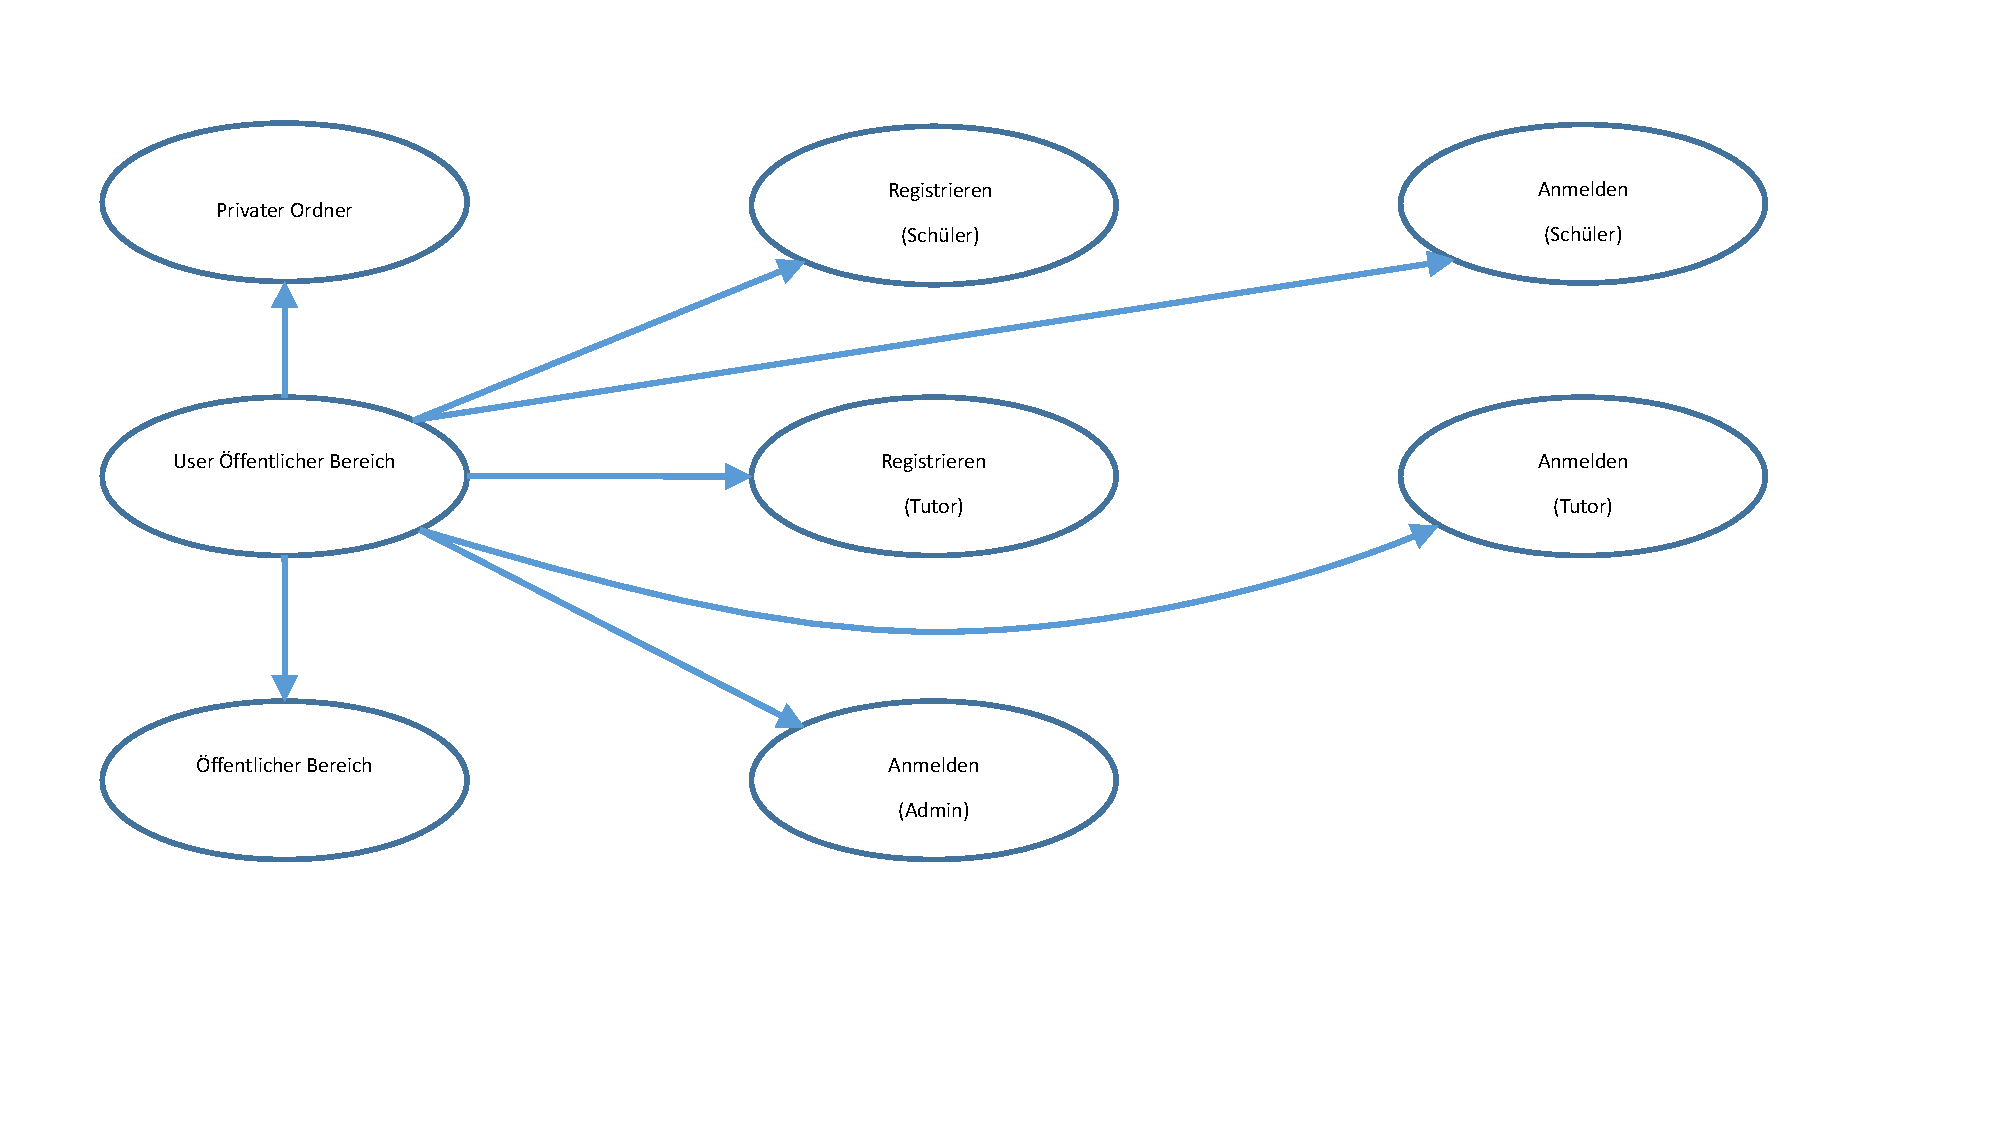
\includegraphics[page=1, width=1\textwidth]{./Source/YWEE_Kontextdiagramm.pdf}}
\caption{Der Besucher der Website hat vollen Zugriff auf den öffentlichen Bereich. Außerdem ist er in der Lage sich als Tutor, Schüler oder Admin anzumelden. Zur Anmeldung des Schülers und Tutors ist eine erfolgreiche Registrierung erforderlich.}
\end{figure}
\newpage
\subsection{Kontextdiagramm Tutor/Schüler/Admin}
\begin{figure}[!htbp]
\fbox{\includegraphics[page=2, width=1\textwidth]{./Source/YWEE_Kontextdiagramm.pdf}}
\caption{Angemeldete Benutzer hingegen haben erweiterte Zugriffsrechte auf diese Funktionen
\newline Grün: erstellen, bearbeiten
\newline Orange: ansehen
\newline Rot: Kontrolle (voller Zugriff)}
\end{figure}

%\section{Glossar}



\end{document}